\begin{bibunit}
\thispagestyle{plain}

% Add missing command definitions from original paper
\newcommand \op[1] {\ensuremath{\operatorname{\mathbf{#1}}}}
\newcommand \com[1] {\ensuremath{\mathtt{#1}}}
\newcommand{\RNum}[1]{\uppercase\expandafter{\romannumeral #1\relax}}

\section*{Abstract}

In this paper, we describe a method to automatically derive the controller for an automated process by an interactive learning approach using a simulation model developed in Visual Components 3D simulation software. The latter is used to record the events of the processes and the controller is generated as an IEC 61499 function block. To create different process scenarios, the actuator signals are triggered manually in appropriate order. The controller logic in Petri net is derived by process discovery algorithms with help of recorded events and conversion of Petri net to IEC 61499 function blocks is done by a software tool configured with a set of transformation rules.
  

\section{Introduction}

Design and validation of Cyber-Physical system’s (CPS) \cite{lee2017introduction}  in industrial automation takes significant time due to the complex interaction of intelligent mechatronic components equipped with embedded control devices. The IEC 61499 standard \cite{iec61499part12012} is considered a suitable approach to design such systems, but the manual development process is still considered to be error-prone, and it takes a lot of development effort. 

Simulation models are very useful for validation, virtual commissioning purposes and to accurately describe the behavior of the automation systems. The controllers can be connected with the simulation models to understand better how the developed control code behaves on it.

In this paper we attempt to go a step further and use simulation models for deriving control code without programming, but as a result of interactive activity. The control code generated from this data-driven approach greatly reduces the engineering effort to program such systems.

The simulation models are easier to interact with than with the real production line. It is possible to record the events that occur in the simulation model. To record the sequence of events, one needs to generate a process scenario and trigger the controller signal manually. The recorded event log is used for the extraction of controller logic with the help of process mining algorithm. The powerful mining tools like ProM \cite{van2005prom}, DISCO \cite{gunther2012disco}, etc., can be of great help to automate this process.

The Visual Components \cite{visualcomponent} 3D simulation software is one of the commercially available tools. The actuator and sensor signals can be manually triggered with the help of this tool. The paper is organized as follows: Section \ref{sec:relatedwork}  discusses the related work and problem statement. Section \ref{sec:methodology} explains the methodology for event log generation, extraction of controller logic in detail. Section \ref{sec:casestudy}  describes the illustrative example of a simulation model and presents the result of the work. Finally, Section \ref{sec:conclusion} concludes the paper and outlines future goals.

\begin{comment}
The Cyber-Physical system’s (CPS) \cite{lee2017introduction}  design and its validation using automation software takes a tremendous amount of time due to the complex  decentralized architecture of embedded devices in each  mechatronic component. The IEC 61499 standard  \cite{iec61499part12012} is considered a suitable approach to design such a system but the development process is still considered to be error-prone and it takes a lot of development effort. The simulation models are very useful for validation and virtual commissioning purposes and it also helps to accurately describe the behavior of the automation systems. . The controllers can be connected with the simulation models  helps to understand 'how the developed control code behaves on it'.  These simulation models can be used for deriving control code without programming, but as a result of interactive activity. The control code generated from this process is less prone to errors and  it greatly reduces the engineering effort to program such as systems. 


The simulation models are considered to be an easier approach to interact with the model rather than with the real production line.  It is possible to record the event that occurs in the simulation model. To record the sequence of events, one needs to generate a process scenario and trigger the controller signal manually instead of using the actual controller. Interactive learning of simulation model is used to record traces of events and we derive the control logic with the help of a process mining algorithm. The powerful mining tools like ProM \cite{van2005prom}, DISCO \cite{gunther2012disco}, etc., can be of great help to automate this process.


The visual components 3D simulation software is considered to be the best approach to  model the system because it gives a better  provision to design , validate and visualize the real  system behavior more precisely compared to the other simulation tools. The actuator and sensor signals can be manually triggered with the help of this tool so as a result, one can get a trace of the desired behavior which can be used to derive control algorithms automatically. In this paper, we propose an interactive learning approach on a simulation model for deriving the control program automatically in IEC 61499 standard with the help of process discovery algorithm. 

The paper is organized as follows: Section \ref{sec:relatedwork}  discusses the related work and problem statement. Section \ref{sec:methodology} explains the methodology for event log generation, extraction of controller logic in detail. Section \ref{sec:casestudy}  describes the illustrative example of a simulation model and presents the result of the work. Finally, Section \ref{sec:conclusion} concludes the paper and outlines future goals.

\end{comment}

\section{Related works and problem statement}
\label{sec:relatedwork}

The process mining technique \cite{10.1007/BFb0101003} \cite{van2012process1} is widely used to extract the business process models and improve the business by analyzing it. The business process models extracted from trace of activities gives a better representation of process scenarios and these models can be used for conformance checking. ProM\cite{van2005prom} is one of the popular open-source tools used for the purpose of discovering the process models, conformance checking, verification of event log, visualization, and simulation of process models. Process mining is not widely explored in the field of industrial control systems but some of the researchers used this for conformance analysis of industrial control systems.


Data and Process Mining Applications on a Multi-Cell Factory Automation Testbed \cite{paper1} explains how process mining can be applied in factory automation. In this approach, industrial control systems record event logs, create a process model using control flow algorithms and then it is used for the improvement of factory automation. Anomaly detection using event log is another area of research that can be applied in industrial control systems and this paper \cite{paper2} describes anomalous activity in the control system by comparing the device log data with the process model. The deviation in event log can be identified by conformance checking and this helps to identify the cyber-attacks in the system. The outlier detection and alarm analysis of industrial plants can be done through the process mining technique \cite{paper3}. The recorded event logs are stored in a database and the model is constructed using a process discovery algorithm. The verification of the event log with respect to the derived process model is used for outlier detection.

Paper \cite{xavier2021plant} explains extraction of the formal model of plant from event logs for the purpose of verification. The formal model of plant from traces expressed in SMV is verified by CTL specifications with the help of NuSMV symbolic model checker. The process mining application is not all explored to derive the control logic or plant model  with the help of recorded events of the system. In this paper, we propose a methodology to derive the control algorithms automatically from the traces of the desired behavior of the system.

\begin{comment}

The process mining technique \cite{10.1007/BFb0101003}  is widely used to extract the business process models and improve the business by analyzing it. The business process models extracted from trace of activities gives a better representation of process scenarios and these models can be used for conformance checking. ProM \cite{van2005prom} is one of the popular open-source tools used for the purpose of discovering the process models, conformance checking, verification of event log, visualization, and simulation of process models. Process mining is not widely explored in the field of  industrial control systems but some of the researchers used this for conformance analysis of industrial control systems. 

Data and Process Mining Applications on a Multi-Cell Factory Automation Testbed \cite{paper1} explains how process mining can be applied in factory automation. In this approach, industrial control systems record event logs , create a process model using control flow algorithms and then it is used for the improvement of factory automation.  Anomaly detection using event log is another area of research that can be applied in industrial control systems and this paper \cite{paper2} describes anomalous activity in the control system by comparing the device log data with the process model. The deviation in event log can be identified by conformance checking and this helps to identify the cyber-attacks in the system.  The outlier detection and alarm analysis of industrial plants can be done through the process mining technique \cite{paper3}.  The recorded event logs are stored in a database and the model is constructed using a process discovery algorithm. The verification of the event log with respect to the derived process model is used for outlier detection.


Paper \cite{xavier2021plant} explains extraction of the formal model of  plant from event logs for the purpose of verification. The formal model of plant from traces expressed in SMV is verified by CTL specifications with the help of NuSMV symbolic model checker. The process mining application is not all explored to derive the control logic or plant model from only with the help of recorded events of the system. In this paper, we propose a methodology to derive the control algorithms automatically from the traces of the desired behavior of the system.

\end{comment}
 
\section{Methodology}
\label{sec:methodology}

\begin{figure}[!t]
	\centering
	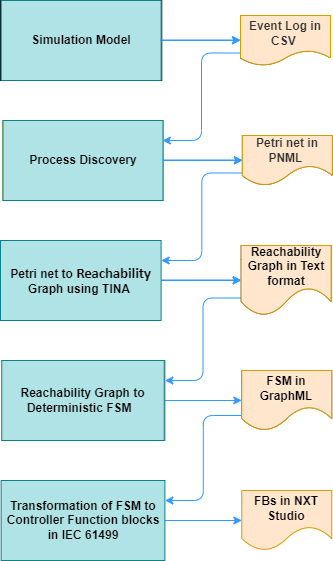
\includegraphics[width=0.3\textwidth]{MX_Papers/Paper6/images/PN2ControllerFlow.png}
	\caption{Methodology}
	\label{Methodology}
\end{figure}

The Figure \ref{Methodology} shows the workflow which starts with recording the events with the help of a simulation model. The user interacts with the simulation model by manually controlling signals and each event occurred in the system is recorded in event log in CSV format. The event log contains the process information about the system, and it is used to extract the process model in terms of Petri net \cite{petri1962} using process discovery algorithm. The Petri net in Petri Net Markup Language (PNML) format is given as input to TINA \cite{berthomieu2004tool} tool for the stepwise simulation and conversion of Petri net to reachability graph. The reachability graph is converted to a deterministic finite state machine and its representation in GraphML helps to visualize the process model and finally the implementation of Controller function block is done with the help of transformation rules. The detailed explanation of the methodology is given in the following subsections  \ref{subsec:eventlog_generation}, \ref{subsec:processdicovery} and \ref{subsec:PNtoIEC61499}.



\subsection{Event log generation}
\label{subsec:eventlog_generation}
The plant model is constructed in the Visual Components 3D environment.  The simulation model works according to the actuator signal values and it shows working behavior of the system as well as the output as sensor values. Here, we are manually changing the actuator signal values and making the system work in accordance with the process scenario. If we want to run a simulation model in a different way, then it is possible to generate such a process scenario by manually triggering the actuator signals. The simulation model developed in the Visual Component tool helps to record these events. The event log records the ’caseId’ for each process run, global state of the system, time and component at which the event occurred, and finally records signal and its corresponding value. The detailed description and representation of example log construction is explained in Section \ref{sec:casestudy}.






\subsection{Process model discovery from event log in terms of Petri net}
\label{subsec:processdicovery}

The recorded event log consists of overall behavior of each process scenario executed in the simulation. To extract the process behavior from the event log, we use process discovery algorithms. Most of the Process discovery algorithms extract the process models in Petri net format \cite{van2013discovering} and it is easy to understand and visualize the system behavior. The alpha algorithm \cite{van2004workflow}  helps to derive the process model from the recorded event log. The ProM tool has several process discovery algorithms so this tool can be used to process create models in form of Petri net. It is also possible to apply the alpha algorithm directly but ProM  helps also in event log pre-processing, model visualization, conformance checking etc. The event log expressed in eXtensible Event Stream (XES) is given as input for the process discovery algorithm and conversion of CSV to XES is done with the help of ProM by mapping standard XES attributes under 'Case' and 'Event' columns.

\subsection{Petri net to IEC 61499 function blocks for controller}
\label{subsec:PNtoIEC61499}

\begin{figure}[!t]
	\centering
	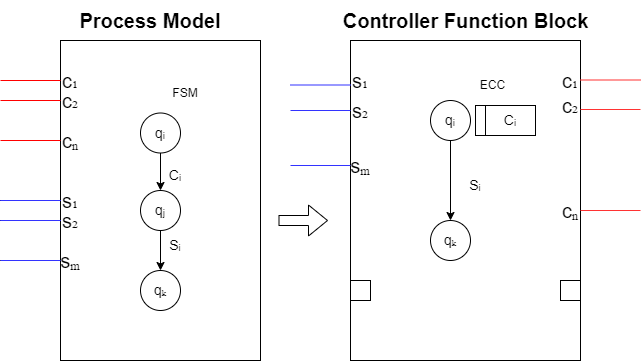
\includegraphics[width=0.5\textwidth]{MX_Papers/Paper6/images/ControlTransformation.png} 
	\caption{Process  Model  to Function Block Interface Transformation }
	\label{ControllerTransformation}
\end{figure}

\begin{figure}[!t]
	\centering
	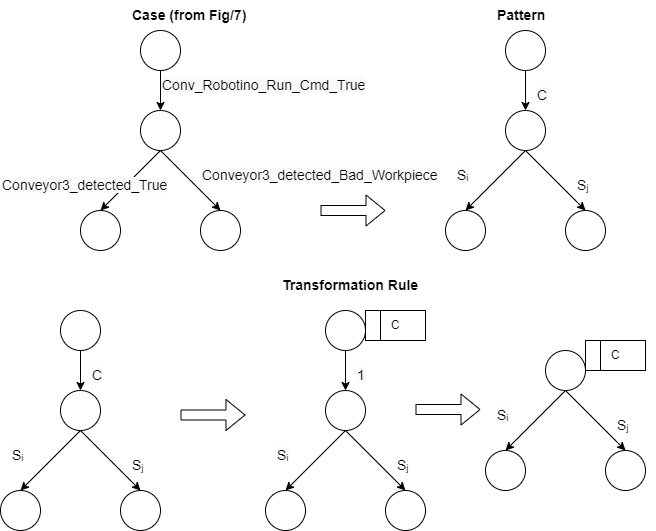
\includegraphics[width=0.5\textwidth]{MX_Papers/Paper6/images/UpdatedControllerConversionrules.png}
	\caption{ FSM to ECC transformation rule}
	\label{conversionrules}
\end{figure}

The Petri net extracted from the event log is used to derive the controller logic and it is  represented as the Execution Control Chart (ECC) of an IEC 61499 function block. 
As a rule, corresponding events are associated with the transitions of Petri nets, which are used to describe processes. The event can be treated as one of the necessary conditions for firing the transition. However, it should be noted that “nameless” transitions are possible in the net model, which can fire spontaneously, without being stimulated by any event.

The reachability graph of a Petri net (if it is finite) is in fact a finite state machine (FSM). When it is constructed for Petri nets describing processes, the FSM can also have spontaneous transitions and, thus, in general the resulting FSM will be a non-deterministic one. To simplify implementation, a non-deterministic FSM should be transform to deterministic one. In this case, determinization will be reduced to getting rid of spontaneous transitions.

The TINA system \cite{berthomieu2004tool} is used to analyze Petri nets and build a reachability graph. It can take Petri net in PNML format as an input and produces the reachability graph in text format. In order to convert the non-deterministic FSM to deterministic FSM and visualize the derived FSM, our software tool called ’Converter of TINA reachability to GraphML’ is used. The deterministic FSM in XML format can be visualized using Gephi \cite{bastian2009gephi} or Yed \cite{wiese2004yfiles} GraphML editors and it represents the whole process workflow of the entire closed-loop system.


\hfill
\subsubsection{TINA reachability graph to GraphML application}
\hfill

\hfill


This methodology can be used for the generation of the plant model and implementation of  the monitor to identify any deviation from the existing process scenario. To incorporate these functionalities later, we need to extend this approach by introducing an  intermediate FSM model (otherwise Petri net can be directly used to generate ECC).

Below the transformation of the textual representation of the reachability graph of a Petri net (which, in fact, is a FSM) in the TINA  modeling system to the GraphML \cite{GraphMLSpec} format used to represent attribute graphs, is considered.

The conversion process can be divided into three phases:

\begin{enumerate}

\item Reading textual input data and generating internal program data structures on their basis. 
\item  Determinization of the FSM.
\item  Generating the output GraphML file.

\end{enumerate}


The presence of the second phase is explained by the fact that so called "spontaneous" transitions can exist in the finite state models. The spontaneous transition is not associated with any input signal and can be activated at any time. In finite automata theory, spontaneous transitions are marked with the symbol $\lambda$ (lambda). In the TINA system, such transitions of Petri nets ported from the ProM system \cite{ProM} are denoted as ‘tau’. A FSM containing spontaneous transitions can be considered non-deterministic, so it becomes necessary to determine it. The advantage of the deterministic FSM is the simplicity of its implementation. In addition, when determining by getting rid of spontaneous transitions, the number of states of the FSM decreases.

In this work, two approaches to the determination of this type are used. The first method is based on the contraction of arcs representing spontaneous transitions, and the second one is based on the reachability principle. The essence of the first approach is as follows: two states connected by a lambda arc are merged into one state. In this case, the incoming and outgoing arcs of both states are combined, and the lambda arc is removed. This rule is applied until there are no lambda arcs left in the converted FSM. However, this method is not universal so it is applicable only in the case of a tree-like topology of lambda arc connection. In the second (universal) method, two states are contracted (merged) into one state only if one state is reachable from another state through a chain of lambda arcs.

The FSM model in TINA is represented as a set of descriptions of states and transitions in a text file with the .kts extension. Each state is described by the following text fragment (in EBNF form):

    
$state <numeric ID of source state>$

trans{$<input signal name>$ / \\ $< numeric identifier of target state>$}

The structure of the description of the FSM model in the GraphML format is as follows. First, there is a description of the attributes of the graph model using the $<key>$ tag, for example:

$<key attr.name="label" id="label" attr.type="string" for="node"/>$

$<key attr.name="Edge Label" id="edgelabel" $\\$ attr.type="string" for="edge"/>4$

In this case, the label attribute of string type is described for graph vertices, as well as the edgelabel attribute of string type is described for graph arcs. Next, there is a set of $<node>$ tags that describe the vertices of the graph. In the automaton interpretation, these vertices are states of the FSM. Example description below:

$<node id="8"><data key="label">$\\$8</data></node>$

To designate transitions (arcs) between automaton states the $<edge>$ tag is used, which contains the following attributes: id is a transition identifier; source is an identifier of the source state of the transition; target is an identifier of the target state of the transition. The $<edge>$ tag has a nested $<data>$ tag that defines the name of the transition. The example of a transition description is below:

$<edge id="8" target="0" source="9">$

$<data key="edgelabel">Repeat</data>$

$</edge>$

To represent the result FB, a special FB markup language is used, described in the second part of the IEC 61499 standard. The $<InterfaceList>$ tag with nested $<EventInputs>$ and $<EventOutputs>$ tags is used to describe a FB interface, which consists of input and output events. A separate event is described by $<Event>$ tag. The $<BasicFB>$ tag describes a basic FB. It has the embedded $<ECC>$ tag corresponding to
an ECC. The ECC, in turn, consists of states ($<ECState>$ tags) and transitions ($<ECTransition>$ tags). Actions in states are defined by $<ECAction>$ tags.


\begin{comment}
The TINA software [] which takes Petri net in PNML format  as an input and produces the reachability graph in text format. The obtained reachability graph can be either deterministic or non-deterministic FSM. In order to convert the non-deterministic FSM to deterministic FSM and visualize the derived FSM, a software tool called 'Converter of TINA reachability to GraphML' [] developed by Dmitry Muromsky is used. The deterministic FSM in XML format can be visualized using Gephi or Yed GraphML editors and it  represents the whole process workflow of the entire closed-loop system.  
\end{comment}

\begin{algorithm}
\caption{FSM to ECC Transformation}\label{alg:two}
\KwData{ $M = (List<States>,List<Arcs>)$ \\ 
$States = \{s_0,s_1,s_2, \dots \}$ \\
$Arcs = \{a_0,a_1,a_2, \dots \}$ \\
$s_i = (name_i, outSignal_i )$ \\
$a_j = (name_j, source_j, target_j)$ \\
$control\_signals = \{c_0,c_1,c_2, \dots \}$ \\}
\KwResult{$TM = (List<States>, List<Arcs>)$}
$TM\_States = \{List<States> \}$ \\
$TM\_Arcs = \{List<Arcs> \}$ \\
\For{ arc in M\_Arcs}{
  $TM\_Arcs.add(arc)$ \\
}
\For{ state in M\_States}{
  $TM\_States.add(state)$ \\
}
\For{ arcs in TM\_arcs}{
 \If{$control\_signals$ has arc.name}{
        $ index\_source = findIndex ( TM\_States => TM\_state.name = arc.source) $ \\
        $ TM\_state[index\_source].outSignal=$\\ $arc.name $ \\

            \For{ arcSource in TM\_Arcs}{
            \If{$arcSource.source =arc.target$}{
            $ arcSource.source \gets arc.source $ \\
            }
        }
          $ TM\_Arcs.remove (arc) $ \\
          $ TM\_States.remove (arc.target) $ \\
    }
}
\end{algorithm}

\hfill
\subsubsection{Transformation of FSM to Controller FB in IEC 61499}
\hfill

The obtained  FSM expressed in GraphML  from the reachability graph consists of a list of states and a list of  edges or arcs.

  \begin{equation}\label{eqn:1}
    M = (List<States>,List<Arcs>)
  \end{equation}
  
Each state consists of a name and output event signal. This output signal is initialized to null and it can be assigned to the control signal while transformation rules are applied. 

  \begin{equation}\label{eqn:2}
    s_i = (name_i, outSignal_i ) 
  \end{equation}
 
 The edge has source state , target state and name (i.e. sensor or actuator signal).
 
   \begin{equation}\label{eqn:3}
     a_j = (name_j, source_j, target_j)
  \end{equation}
 
 To derive the controller logic, we need to apply the transformation rules on top of the derived FSM. Whenever an actuator signal value occurs at the edge of FSM then the following rules are applied.


\begin{itemize}
  \item The corresponding edge and its target state are removed from the ECC.
  \item  Actuator signal triggers as an output event at the source state of the removed edge
  \item The edge starts from the removed state  is connected back to the source state of removed edge.
\end{itemize}


The interface of the controller is shown in the Figure \ref{ControllerTransformation}. Controller function block takes all sensor signals as input events and  produces actuator signals as output. The FSM of the process model is converted to ECC using the transformation rule. If control signal $C_i$ is triggered from state $q_i$ to $q_k$ then the  state $q_j$ is removed  from ECC  and state $q_i$ produces $c_i$ event. 


The Figure \ref{conversionrules} explains the FSM to ECC transformation with the help of an example case from Figure \ref{SIM_Yed}.  The Conv\_Robotino\_Run\_Cmd\_True is a control signal and FSM takes different paths according to the sensor values of the Conveyor3\_detected\_True and Conveyor3\_detected\_Bad\_Workpiece and this pattern is expressed in the Figure \ref{conversionrules}. When the control signal appears on the edges of the FSM  then the rule is straight-forward i.e. control signals replaced by '1' signal and their respective output place produce corresponding control signal as output. It is possible to simplify the ECC further  by removing edges with condition  “1” or “True” and its target state. The transformation from FSM to ECC is represented as the Algorithm \ref{alg:two}.



\section{case study : Automatic generation of controller by interactive learning}
\label{sec:casestudy}

\begin{figure}[!t]
	\centering
	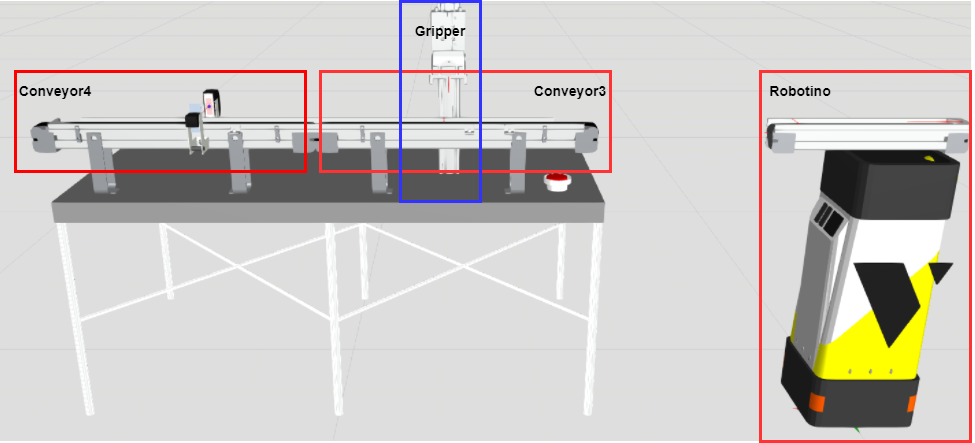
\includegraphics[width=0.5\textwidth]{MX_Papers/Paper6/images/simulation.png}
	\caption{Simulation in Visual Components}
	\label{SIM_UI}
\end{figure}

\subsection{General Description of simulation in Visual Components' 3D environment}

The plant model constructed in Visual Components 3D manufacturing simulation software tool is shown in the Figure \ref{SIM_UI}.	The production system consists of a conveyor line, composed of 2 conveyor sections ( conveyor3 and conveyor4 ), gripper and autonomous guided vehicle Robotino with a conveyor section mounted on top.  Conveyor1 and Conveyor2 are not connected to the production line and never used in this experiment.

There are six actuators and four sensors on the production system. The conveyor line composed of Conveyor3 and  Conveyor4  has  one actuator each for  to run the conveyor i.e. $Conveyor3\_run\_cmd = True$ for starting the conveyor  and $Conveyor3\_run\_cmd = False$ to stop it. Likewise,  Conveyor3 and  Conveyor4  have  one sensor each for  detecting workpiece ($ Conveyor3\_detected$ and $camera1\_sensor\_c4\_detected$). The Gripper component can move upwards and downwards with help of $Gripper1\_extend\_cmd$. In order to grab and release  the workpiece, the Gripper component uses the $Gripper1\_close\_cmd$ actuator signal. It consists of two sensors, the $Gripper1\_extended$ sensor  which helps to determine whether the gripper extended or not and the $Gripper1\_closed$ sensor to identify whether the workpiece is released or not. Robotino component creates a workpiece ( a 3D object looks like a cup) and connects with the conveyor line to transfer the workpiece for further processing. The following table shows all actuator and sensor signals used for this experiment.

\hfill

\begin{tabularx} {0.45\textwidth} { 
   | >{\raggedright\arraybackslash}X 
  | >{\centering\arraybackslash}X 
  | >{\raggedleft\arraybackslash}X | }
 \hline
 
 Actuator signals  \\
 \hline

Conveyor\_Robotino\_run\_cmd\_True \\
Conveyor\_Robotino\_run\_cmd\_False \\
Conveyour3\_run\_cmd\_True \\
Conveyour3\_run\_cmd\_False \\
Conveyor\_Robotino\_create\_new\_cup\_cmd\_True \\
Conveyor\_Robotino\_create\_new\_cup\_cmd\_False \\
Gripper1\_extend\_cmd\_True \\
Gripper1\_extend\_cmd\_False \\
Conveyour4\_run\_cmd\_True \\
Conveyour4\_run\_cmd\_False \\
Gripper1\_close\_cmd\_True \\
Gripper1\_close\_cmd\_False \\

\hline
 Sensor signals  \\
\hline
Conveyour3\_detected\_BadWorkPiece \\
Conveyour3\_detected\_True \\
Conveyour3\_detected\_False \\
Camera1\_sensor\_c4\_detected\_empty \\
Gripper1\_extended\_30.0 \\
Gripper1\_opened\_5.0 \\
Gripper1\_vertical\_retracted\_0.0 \\
Gripper1\_closed\_0.0 \\
\hline


\end{tabularx}
\\

The 3D view in simulation gives better understanding about the system's behavior. It is possible to construct different processing traces by manipulating the  actuator signals. This plant has two processing scenarios, the first scenario explains normal behavior of the system whenever a work piece arrives and the second one describes how the plant reacts whenever a bad work piece is detected.

The  processing sequence of the plant is as follows: 

\begin{enumerate}

  \item Robotino creates a new 3D object of the workpiece (i.e. structure like a cup) and it transfers the workpiece to the conveyor3.  
  \item Conveyor3 starts running and stops at the point where Gripper can grab the workpiece. Gripper processes the workpiece and places it back to the conveyor3 and then the conveyor starts running, transferring the workpiece to conveyor4 and this process is repeated in a cyclic order.
  \item Whenever a bad workpiece is detected then Gripper does not perform any actions.
\end{enumerate}




\subsection{Event log Description}


\begin{figure}[!t]
	\centering
	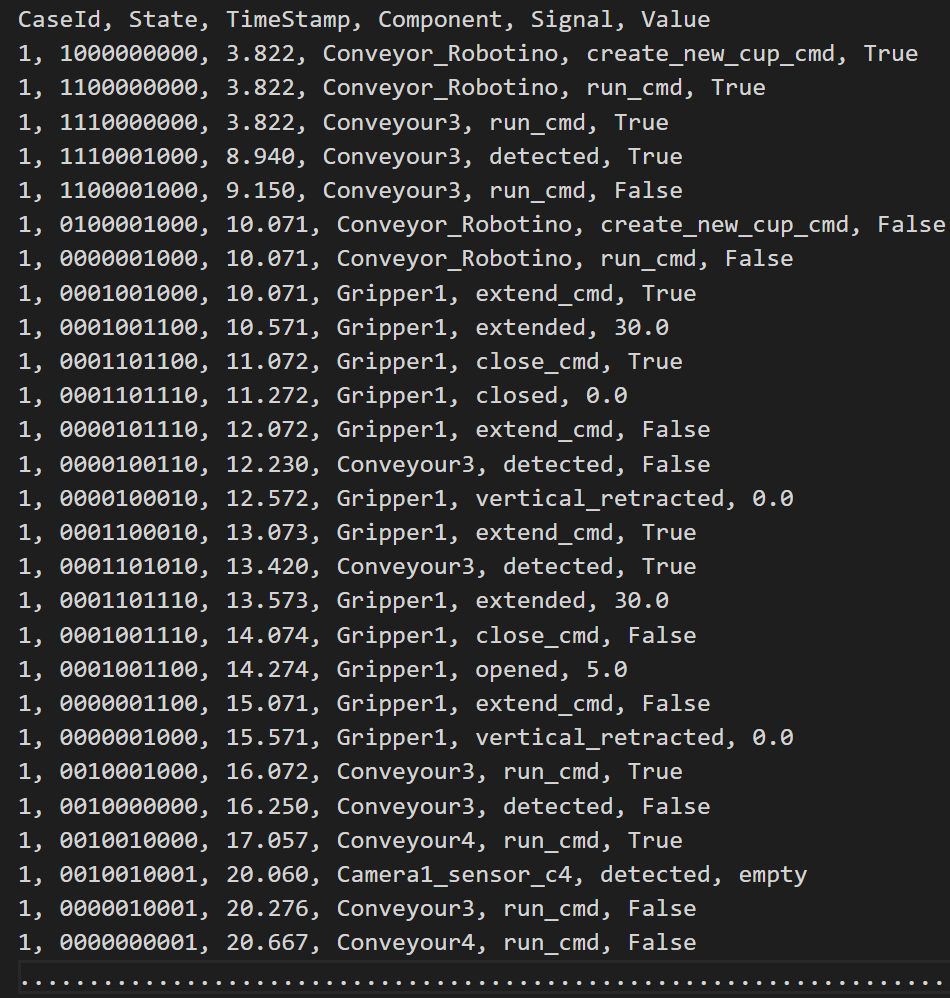
\includegraphics[width=0.5\textwidth]{MX_Papers/Paper6/images/EL1.PNG}
	\caption{Event log}
	\label{SIM_EL}
\end{figure}

\begin{figure*}[!t]
	\centering
	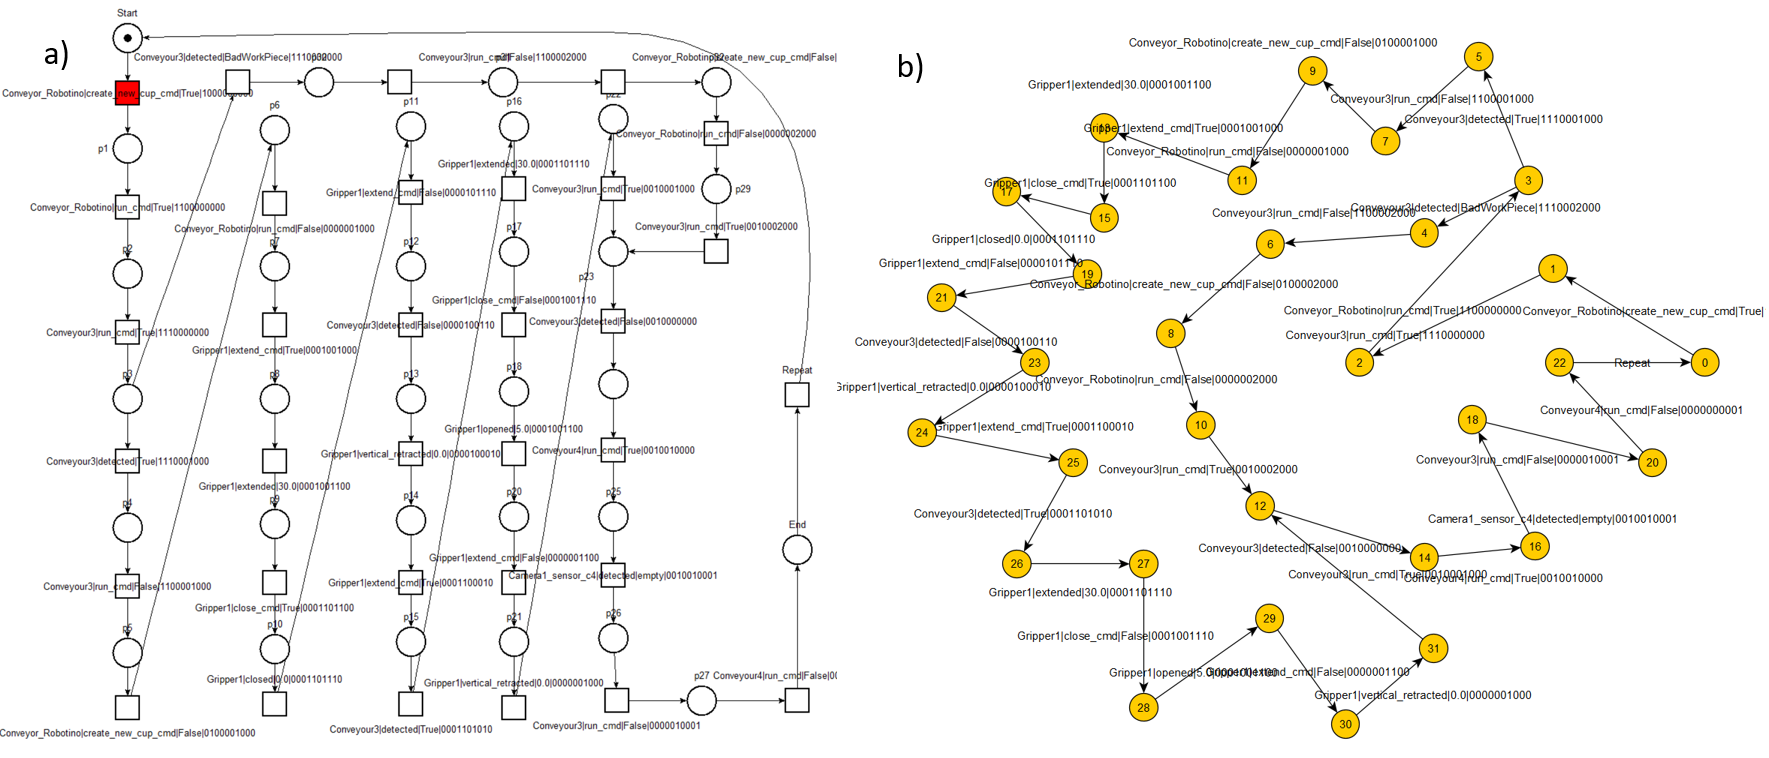
\includegraphics[width=1\textwidth]{MX_Papers/Paper6/images/PNFSMPNG.PNG}
	\caption{a) The Petri net during its step-wise simulation observation b) The obtained FSM from Petri net}
	\label{SIM_Yed}
\end{figure*}


The different traces in the event log are generated by following appropriate triggering of actuator signals manually. These events are recorded in CSV format as shown in the Figure \ref{SIM_EL} and it consists of six columns: CaseId, State, TimeStamp, Component, Signal and Value. CaseId is unique for each processing sequence scenario, State is the encoded combination signal values of sensors and actuators, TimeStamp represents the time at which the event is triggered and finally, the combination of Component, signal and value column helps to form a complete description of an activity of an event. The State is a string value constructed by joining the encoded signal values of sensors and actuators and it helps to determine the unique status of the system. The event log is sorted according to the timestamp and is taken for the further process. The event log expressed in CSV format is converted to XES format because most of the process discovery algorithms accept this format. To convert CSV to XES format, it is necessary to specify the ’Case’ and ’Event’ columns. The ’Case’ column is  selected as ’CaseId’ and the combination of component, signal, value and state as the ’Event’ column.

\subsection{FSM generation from event log}



The process discovery method is used to identify the behavior of the system. In order to extract the process from the system, the process mining algorithm called alpha  is applied on top of the recorded event log and it converts the process sequences to  a Petri net. The obtained Petri net is shown in Figure \ref{SIM_Yed} (a) during its step-wise simulation observation. The initial marking on ’Start’ place is added for the simulation and conversion purpose of Petri net. To achieve the process to run in cyclic, a new transition ’Repeat’ is added  which connects from ’End’ to ’Start’. The finite reachability graph can be considered as a Finite State Machine and the TINA tool helps to construct the reachability graph from the Petri net and save it in text format. The reachability graph expressed in text format is converted to deterministic FSM in GraphML format is done with help of our software tool 'TINA reachability graph to GraphML application'. FSM representation can be edited or visualized with help of GraphML editor tools like Gephi, Yed etc. The FSM representation in Yed GraphML editor is shown in the Figure \ref{SIM_Yed} (b). The obtained FSM consists of two loops: First loop explains normal working behavior of the plant and the second one is the shorter one that explains ’How does the system behave whenever a bad workpiece arrives?’ and the ’Repeat’ signal makes the FSM run in cycles.
 


\subsection{IEC 61499 representation of Controller}

\begin{figure*}[!t]
	\centering
	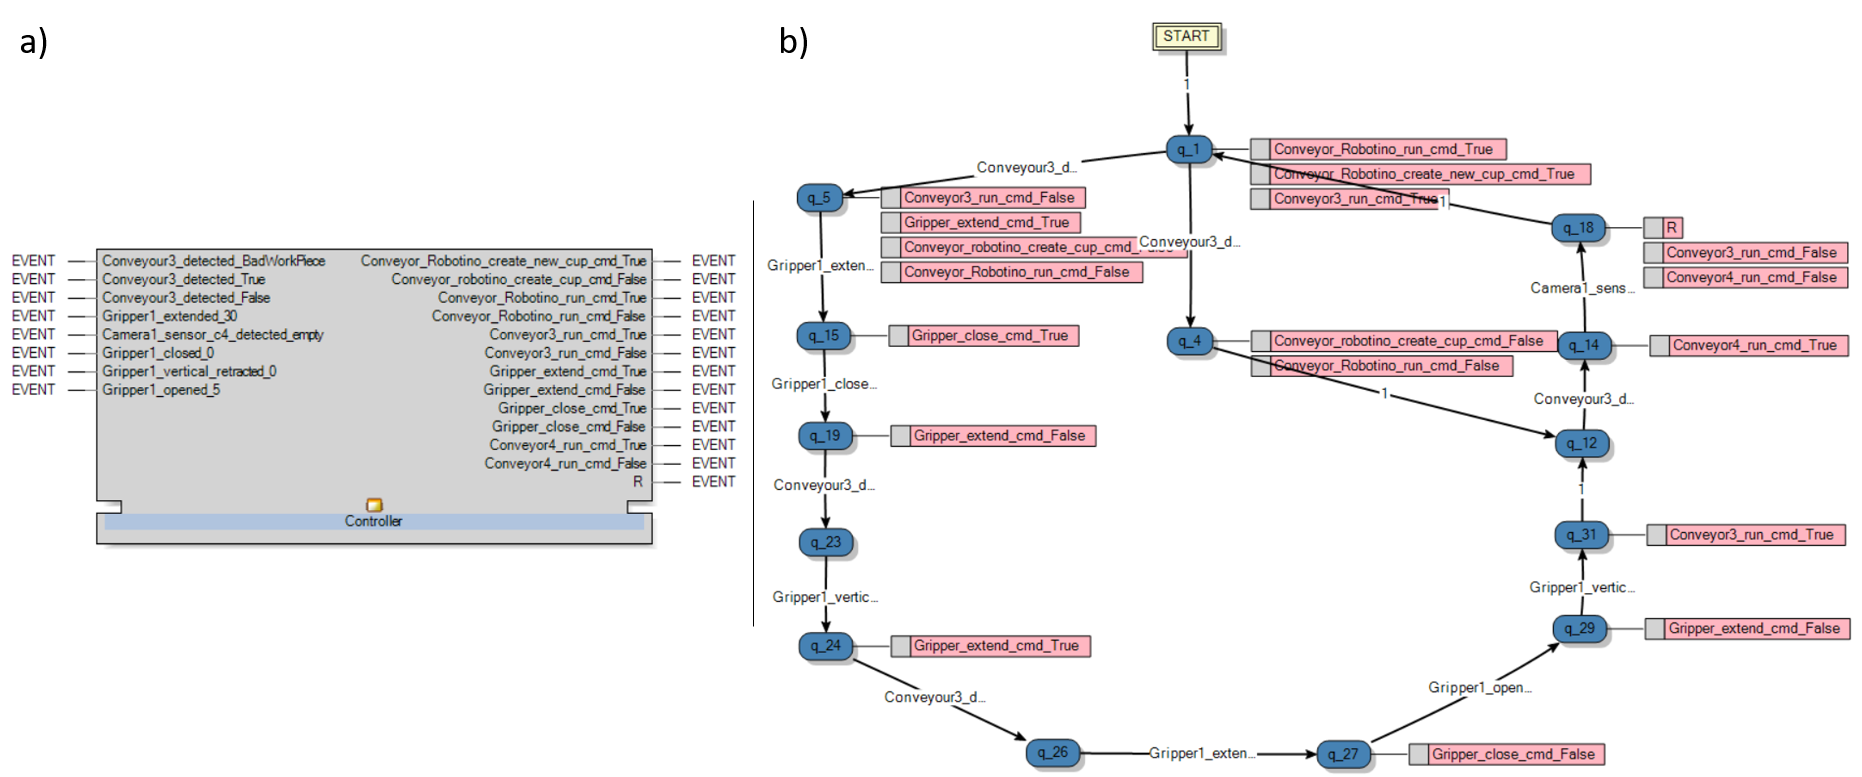
\includegraphics[width=1\textwidth]{MX_Papers/Paper6/images/FB.PNG}
	\caption{a) Function block interface of Controller b) ECC representation in of Controller}
	\label{SIM_CON_ECC}
\end{figure*}


The FSM extracted from the event log describes the whole system behavior. To derive the controller in IEC 61499 standard, we use the transformation rules that were discussed earlier. The IEC 61499 function block interface of the controller is shown in the Figure \ref{SIM_CON_ECC} (a). It consists of sensor signals as input events and actuator signals as output events. The 'State' string can be neglected because it was used to identify the unique state in FSM.  The ECC of the controller is shown in the Figure  \ref{SIM_CON_ECC} (b). Whenever any actuator signal appears on the edges of FSM is transformed as output events and sensor signals remain the same as condition in ECC. The consecutive edges without any conditions in ECC (i.e. ideally "True" or "1" condition)   can be merged into the common state and all actuator signals can be expressed as  events in a separate 'Action' of ECC. The event 'Repeat' is changed to 'R' because 'Repeat' is a keyword in NxtStudio software. 





\section{Conclusion and Future Work}
\label{sec:conclusion}


The interactive learning approach helps to create controller in IEC 61499 function block automatically. The developed approach gives promising results. The process logic expressed in FSM helps to understand the process in a better way.  The working of the same simulation model under different process scenarios can be implemented as a different controller function block. It is possible to drive  the system by activating the actuator signals and this simple approach helps in deriving the same process logic.  


The proposed approach requires the global state information of the system and it needs to be recorded on the event log whenever an event occurs. It is difficult to get a ‘snapshot’ of the states of all sensors when there is a current active event.  To do this, we must poll all sensors but there will be considerable time delays in the transmission of the information via the network, so the data read from the sensors will be marked with different timestamps than the event’s timestamp. The distributed controllers in the network consist of synchronized clocks with all the sensor readings where time stamped could be used but this makes the system more complex and sensor polling time delays remain the same. 


This approach needs to  be validated and tested in different simulation models or even in real systems to determine the accuracy of the extracted controller logic. The development of optimal ECC of complex systems consisting of multiple controllers is considered as the next step in the future. Formal verification of the system helps to identify the possible errors before deploying an automatically generated controller on the real system. The IEC 61499 formal verification tool chain \cite{xavier2021cyber} integrated with the proposed approach can be used for automatic verification and validation using specifications.


\section{Acknowledgements}
This work was sponsored, in part, by the H2020 project 1-SWARM co-funded by the European Commission (grant agreement: 871743). We are also thankful to Visual Componenets (https://www.visualcomponents.com/) for providing with licenses for the 3D simulation tool.

\clearpage
\putbib
\end{bibunit} 